\documentclass{amsart}

% === TITLE === (((
\title{Representing Convex Structures with Chess}
\keywords{Convex structure, chess.}
% )))

% === PACKAGES === (((
\usepackage{amsmath}
\usepackage{amsfonts}
\usepackage{amssymb}
\usepackage{mathrsfs}
\usepackage{graphicx}
% )))

% === AUTHORS === (((
%    author one information
\author{Esteban Lluis-Aceff}
\address{CDMX. Mexico}
\curraddr{14100, Mexico}
\email{esteban@xeleva.com}
% \thanks{Jorge Macías Díaz.}

%    author two information
\author{Erick I. Rodríguez-Juárez}
\address{CDMX. Mexico}
\curraddr{Mexico}
\email{nijerc@gmail.com}
% \thanks{Omar Antolín Camarena.}
% \subclass[2010]{Primary }
% )))

% === ENVIRONMENTS === (((
\newtheorem{theorem}{Theorem}[section]
\newtheorem{prop}[theorem]{Proposition}
\newtheorem{lemma}[theorem]{Lemma}
\newtheorem{coro}[theorem]{Corollary}

\theoremstyle{definition}
\newtheorem{definition}[theorem]{Definition}
\newtheorem{example}[theorem]{Example}
\newtheorem{xca}[theorem]{Exercise}

\theoremstyle{remark}
\newtheorem{remark}[theorem]{Remark}

\numberwithin{equation}{section}
% )))

% === COMMANDS === (((
\newcommand{\dis}{\displaystyle}
% )))

\begin{document}

% === ABSTRACT === (((
\maketitle
\begin{abstract}
\end{abstract}
% )))

\section{Introduction} % (((
% )))

\section{Notation} % (((
% )))

\section{Moore Families} % (((
\begin{definition}
Let \(X\) be a set.
Let \(\mathscr{C} \subseteq \mathscr{P} (X)\).
We call \(\mathscr{C}\) a \textbf{Moore family} if and only if
the following conditions are satisfied:
\begin{enumerate}
	\item \(\varnothing , X \in \mathscr{C}\).
	\item \(\forall \mathscr{D} \subseteq \mathscr{C} \left(
	(\mathscr{D} \ne \varnothing) \;\implies\; 
	\dis\bigcap \mathscr{D} \in \mathscr{C}\right)\)
\end{enumerate}
\end{definition}

\begin{definition}
Let \(X\) be a set.
Let \(\alpha : \mathscr{P} (X) \longrightarrow \mathscr{P} (X)\).
We call \(\alpha\) a \textbf{closure operator} if and only if
the following conditions are satisfied:
\begin{enumerate}
	\item \(\alpha (\varnothing) = \varnothing\).
	\item \(\forall A \in \mathscr{P} (X) (A \subseteq \alpha (A))\).
	\item \(\forall A,B \in \mathscr{P} (X) (A \subseteq B \;\implies\; 
	\alpha (A) \subseteq \alpha (B))\).
	\item \(\forall A \in \mathscr{P} (X) (\alpha (\alpha (A)) = A)\).
\end{enumerate}
\end{definition}

\begin{definition}
We denote
\[
\begin{array}{rcl}
MF_X & = & \{
	\mathscr{D} \subseteq \mathscr{P} (X) :
	\mathscr{D} \mbox{ is a Moore family}
\}, \\ 
CL_X & = &  \{
\alpha \in \mathscr{P}(X) ^{ \mathscr{P} (X)} :
\alpha \mbox{ is a closure operator}
\}.\\
\end{array}
\]
\end{definition}

\begin{lemma}
Let \(\alpha \in CL_X\).
Then 
\begin{enumerate}
\item[(a)] \(Im (\alpha) \in MF_X\). 
\item[(b)] \(\forall \mathscr{D} \subseteq Im(\alpha)\),
\(A = \dis\bigcap \mathscr{D}\) is such that \(\alpha (A) = A\).
\end{enumerate}
\label{image:lem}
\end{lemma}
\begin{proof}
We verify that \(Im(\alpha) \in MF_X\).
\begin{enumerate}
\item
\(\varnothing = \alpha (\varnothing) \in Im(\alpha)\), and 
\(X \subseteq \alpha (X) \subseteq X \implies X = \alpha (X) \in Im(\alpha)\)
\item 
Let \(\varnothing \neq \mathscr{D} \subseteq Im (\alpha)\). 
Define \(A = \dis\bigcap \mathscr{D}\).
We must have \(A \in Im (\alpha\)). \\ 
Notice that, \(\forall Z \in \mathscr{D} \subseteq Im(\alpha)\), 
\(\exists B \in \mathscr{P} (X)\) such that \(Z = \alpha (B)\). 
Then
\[
\alpha (Z) = \alpha (\alpha (B)) = \alpha (B) = Z.
\]
Let \(Z \in \mathscr{D}\). 
Then \(A \subseteq Z\), and \(\alpha (A) \subseteq \alpha (Z)\).
Therefore
\[
A \subseteq \alpha (A) \subseteq \dis\bigcap_{Z \in \mathscr{D}} \alpha (Z) 
= \dis\bigcap_{Z \in \mathscr{D}} Z = A.
\]
Finally \(A = \alpha (A) \in Im(\alpha)\), which proves (a) and (b).
\end{enumerate}
\end{proof}

\begin{lemma}
Let \(\mathscr{D} \in MF_X\). 
Then \(\Phi _{\mathscr{D}} : \mathscr{P} (X) \longrightarrow \mathscr{P} (X)\) 
defined by
\[
\Phi _{\mathscr{D}} (A) 
= \dis\bigcap_{\stackrel{Z \in \mathscr{D}}{A \subseteq Z}} Z,
\]
is such that \(\Phi _{\mathscr{D}} \in CL_X\).
\label{well_defined:lem}
\end{lemma}
\begin{proof}
\begin{enumerate}
\item
\label{empty:enu}
\(\Phi _{\mathscr{D}} (\varnothing) 
= \dis\bigcap_{\stackrel{A \in \mathscr{D}}{\varnothing \subseteq A}} A 
= \varnothing\).
\item
\label{extensive:enu}
Let \(A \in \mathscr{P} (X)\). 
We will show that \(A \subseteq \Phi _{\mathscr{D}} (A)\). \\ 
Let \(a \in A\), and \(Z \in \mathscr{D}\), such that \(A \subseteq Z\).
Then \(a \in Z\), and
\[
	\therefore \hspace{5mm}
	a \in \dis\bigcap_{\stackrel{Z \in \mathscr{D}}{A \subseteq Z}} Z
	\;\implies\; 
	A \subseteq \dis\bigcap_{\stackrel{Z \in \mathscr{D}}{A \subseteq Z}} Z
	= \Phi _{\mathscr{D}} (A).
\]
\item
\label{monotone:enu}
Let \(A,B \in \mathscr{P} (X)\), such that \(A \subseteq B\).
We require \(\Phi _{\mathscr{D}} (A) \subseteq \Phi _{\mathscr{D}} (B)\).\\ 
Notice that
\(\{Z \in \mathscr{D} \;:\; B \subseteq Z\} 
\subseteq \{Z \in \mathscr{D} \;:\; A \subseteq Z\}\).
Therefore,
\[
	\Phi _{\mathscr{D}} (A) 
	= \dis\bigcap_{\stackrel{Z \in \mathscr{D}}{A \subseteq Z}} Z 
	\subseteq \dis\bigcap_{\stackrel{Z \in \mathscr{D}}{A \subseteq Z}} Z
	= \Phi _{\mathscr{D}} (B).
\]
\item
\label{idempotent:enu}
We need to show \(\Phi _{\mathscr{D}} (A) 
= \Phi _{\mathscr{D}} (\Phi _{\mathscr{D}} (A))\).
By (2), \(\Phi _{\mathscr{D}} (A) 
\subseteq \Phi _{\mathscr{D}} (\Phi _{\mathscr{D}} (A))\). \\
Let \(Z_0 \in \mathscr{D}\) such that \(A \subseteq Z_0\). 
Therefore 
\(
\Phi _{\mathscr{D}} (A) 
= \dis\bigcap_{\stackrel{Z \in \mathscr{D}}{A \subseteq Z}} Z 
\subseteq Z_0.
\)
\[
\begin{array}{rrcl}
\therefore & 
\forall Z \in \mathscr{D} (A \subseteq Z 
& \implies &
\Phi _{\mathscr{D}} (A) \subseteq Z) \\ 
\therefore & 
\{Z \in \mathscr{D} \;:\; A \subseteq Z\} 
& \subseteq &
\{Z \in \mathscr{D} \;:\; \Phi _{\mathscr{D}} (A) \subseteq Z\} \\ 
\therefore & 
\Phi _{\mathscr{D}} (\Phi _{\mathscr{D}} (A)) =
\dis\bigcap_{\stackrel{Z \in \mathscr{D}}{\Phi _{\mathscr{D}} (A) \subseteq Z}}Z
& \subseteq & 
\dis\bigcap_{\stackrel{Z \in \mathscr{D}}{A \subseteq Z}} Z
= \Phi _{\mathscr{D}} (A).
\end{array}
\hspace{1cm}
\]
\end{enumerate}
\end{proof}

\begin{lemma}
	Let \(\mathscr{D} \in MF_X\).
	Then 
	\(Im(\Phi _{\mathscr{D}}) = \mathscr{D}\).
	\label{onto:lem}
\end{lemma}
\begin{proof}
	% Since \(\mathscr{D} \in MF_X\), then
	% \(Im(\Phi _{\mathscr{D}}) \subseteq \mathscr{D}\).
	Since \(\mathscr{D} \in MF_X\),
	\(\forall A \subseteq X \),
	\(\Phi _{\mathscr{D}} (A)
	% = \dis\bigcap_{\stackrel{Z \in \mathscr{D}}{A \subseteq Z}} Z 
	\in \mathscr{D}\).
	Then \(Im(\Phi _{\mathscr{D}}) \subseteq \mathscr{D}\).
	% We prove \(\mathscr{D} \subseteq Im(\Phi _{\mathscr{D}})\).
	Let \(A \in \mathscr{D}\).
	So \(A \in \mathscr{D}\) is such that \(A \subseteq A\),
	\(
	A \subseteq 
	\Phi _{\mathscr{D}} (A) =
	\dis\bigcap_{\stackrel{Z \in \mathscr{D}}{A \subseteq Z}} Z 
	\subseteq A
	\). 
	Then \(A = \Phi _{\mathscr{D}} (A)\), and 
	\(\mathscr{D} \subseteq Im(\Phi _{\mathscr{D}})\).
\end{proof}

\begin{prop}
Let \(\Phi  : MF_X \longrightarrow CL_X\) be defined by:
\[
\Phi  _ {\mathscr{D}} : 
\mathscr{P} (X) \longrightarrow \mathscr{D} \;,\; 
\Phi _{\mathscr{D}} (A) = 
\dis\bigcap_{\stackrel{Z \in \mathscr{D}}{A \subseteq Z}} Z.
\]
Then \(\Phi\) is a bijection.
\label{bijection:prop}
\end{prop}
\begin{proof}
We prove injection. Let \(\mathscr{C} , \mathscr{D} \in MF_X\), such that
\(\Phi _{\mathscr{C}} = \Phi _{\mathscr{D}}\). By Lemma \ref{onto:lem},
\[
\mathscr{C} = Im (\Phi _{\mathscr{C}}) = Im (\Phi _{\mathscr{D}}) = \mathscr{D}.
\]
It remains verify surjection. Let \(\alpha \in CL_X\).
Consider \(\Phi _{Im(\alpha)} : \mathscr{P} (X) \longrightarrow Im(\alpha)\).
	By Lemma \ref{image:lem}(a), \(Im(\alpha) \in MF_X\).
Let \(A \subseteq X\).
Notice that \(A \subseteq \alpha (A) \in Im(\alpha)\).
\[
\begin{array}{c}
\therefore \hspace{5mm} A \subseteq \Phi _{Im(\alpha)} (A) =
\dis\bigcap_{\stackrel{Z \in Im(\alpha)}{A \subseteq Z}} Z
\subseteq \alpha (A)
\\ 
\therefore \hspace{5mm} 
\alpha (A) 
\subseteq \alpha \big(\Phi _{Im(\alpha)} (A)\big) 
\subseteq \alpha (\alpha (A)) 
= \alpha (A)
\;\implies\; 
\alpha (\Phi _{Im(\alpha)} (A)) = \alpha (A).
\end{array}
\]
Since \(\mathscr{D}' = 
\{Z \in Im(\alpha) : A \subseteq Z\} \subseteq Im(\alpha)\),
then \(\Phi _{Im(\alpha)} (A) = \dis\bigcap \mathscr{D}'\). \\ 
Applying the Lemma \ref{image:lem}(b) to \(\alpha \in CL_X\),
and \(\Phi _{Im(\alpha)} (A) = \dis\bigcap \mathscr{D}'\), we obtain
\[
\alpha (A) = \alpha (\Phi _{Im(\alpha)} (A)) 
= \Phi _{Im(\alpha)} (A)
\;\implies\; 
\Phi _{Im(\alpha)} = \alpha .
\]
\end{proof}

% \begin{remark}
% We have shown
% \begin{enumerate}
% \item 
% \(\Phi^ {-1} (\alpha) = Im (\alpha)\).
% \item 
% For every \(\alpha \in CL_X\),
% \(\alpha (A) = 
% \dis\bigcap_{\stackrel{Z \in Im(\alpha)}{A \subseteq Z}} Z\).
% \end{enumerate}
% \end{remark}
% )))

\section{Convex Structures} % (((
\begin{definition}
Let \(X\) be set.
Let \(\mathscr{C} \subseteq \mathscr{P} (X)\).
We call \(\mathscr{C}\) a \textbf{convex structure} if and only if
the following conditions are satisfied:
\begin{enumerate}
	\item \(\varnothing , X \in \mathscr{C}\).
	\item \(\forall \mathscr{D} \subseteq \mathscr{C}
	\left(\mathscr{D} \ne \varnothing
		 \;\implies\; \dis\bigcap \mathscr{D} \in \mathscr{C} \right)\).
	\item \(\forall \mathscr{D} \subseteq \mathscr{C} \left(
	\forall D_1,D_2 \in \mathscr{D} (D_1 \subseteq D_2 \lor D_2 \subseteq D_1 )
	\;\implies\; \dis\bigcup \mathscr{D} \in \mathscr{C} 
	\right)\)
\end{enumerate}
\end{definition}

\begin{definition}
We call \(\alpha : \mathscr{P} (X) \longrightarrow \mathscr{P} (X)\) a 
\textbf{domain finite} or \textbf{algebraic} if and only if
\[
	\forall A \in \mathscr{P} (X)
	\left(
	\alpha (A) = \dis\bigcup_{F \in [A] ^{< \aleph _0}} \alpha (F)
	\right).
\]
\end{definition}

\begin{definition}
	Let
	\[
		\begin{array}{rcl}
		CS_X & = & 
		\{\mathscr{C} \subseteq \mathscr{P} (X) \;:\; \mathscr{C} 
		\mbox{ is a convex structure} \},
		\\
		CLA_X & = & 
		\{\alpha  \in \mathscr{P} (X) ^ {\mathscr{P} (X)} \;:\; 
			\alpha \mbox{ is an algebraic closure operator}\}.
		\end{array}
	\]
\end{definition}

\begin{lemma}
Let \(X\) be a set.
Let \(\mathscr{C} \subseteq \mathscr{P} (X)\) be a convex structure.
Then
\[
	F \in \Big[\dis\bigcup \mathscr{C}\Big] ^ {< \aleph _0} \iff 
	\exists Z \in \mathscr{C} (F \in [Z]^ {< \aleph _0}).
\]
\end{lemma}

\begin{theorem}[\cite{van}]
\(\Phi _{\mathscr{D}} \in CLA_X \iff \mathscr{D} \in CS_X\).
\end{theorem}
\begin{proof}
Let \(\mathscr{D} \in MF_X\).
We note that \(\mathscr{D} = Im(\Phi _{\mathscr{D}})\). \\ 
We must verify that \(\mathscr{D}\) is closed under unions of chains. \\ 
Let \(\mathscr{C} \subseteq \mathscr{D}\) a chain. 
Let \(Z \in \mathscr{C}\), then 
\(Z = \dis\bigcup_{F \in [Z]^ {< \aleph _0}} \Phi _{\mathscr{D}} (F)\). 
	\begin{figure}[hbtp!]
		\centering
		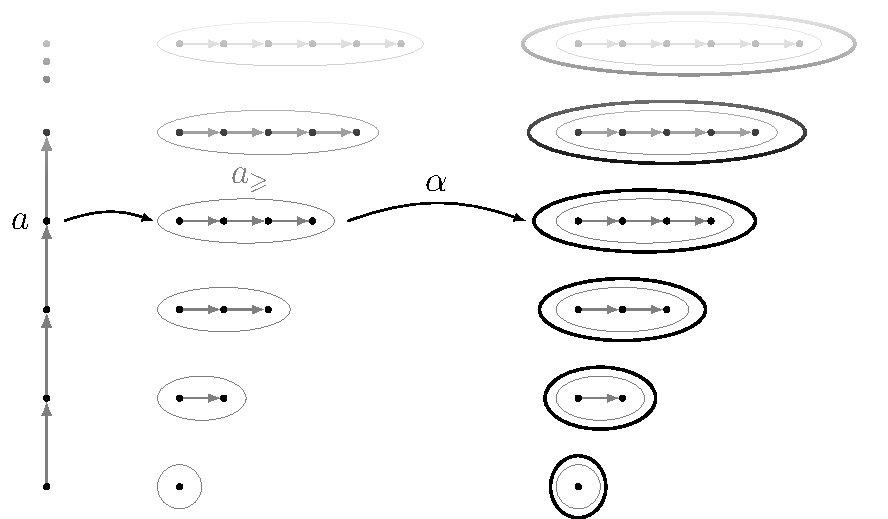
\includegraphics[width= 0.6 \linewidth, page = 1]{IMAGES/2/2}
	\end{figure}
\newpage % just to set the image
Therefore
\[
	\dis\bigcup \mathscr{C} =
	\dis\bigcup_{Z \in \mathscr{C}} 
	\dis\bigcup_{F \in [Z]^ {< \aleph _0}} \Phi _{\mathscr{D}} (F).
\]
(incomplete)
\end{proof}
% )))

\section{Finite Convex Structures} % (((
% )))

\section{Chess} % (((
% )))

\section{Further Work} % (((
% )))

% === REFERENCES === (((
\bibliography{References}
\bibliographystyle{unsrt}
% )))

\end{document}
